\chapter{Estado del arte}
Aplicaciones existentes para aprender programación orientada a objetos:
% Please add the following required packages to your document preamble:
% \usepackage[table,xcdraw]{xcolor}
% If you use beamer only pass "xcolor=table" option, i.e. \documentclass[xcolor=table]{beamer}
% \usepackage{longtable}
% Note: It may be necessary to compile the document several times to get a multi-page table to line up properly
\begin{longtable}[c]{|l|l|l|l|l|l|}
\caption{My caption}
\label{my-label}\\
\hline
\rowcolor[HTML]{34CDF9} 
{\color[HTML]{FFFFFF} Nombre}                                              & {\color[HTML]{FFFFFF} Temas}                                                                                                                                                                                                                                                                                                                                                                                                 & {\color[HTML]{FFFFFF} Juegos} & {\color[HTML]{FFFFFF} Tamaño} & {\color[HTML]{FFFFFF} Idioma} & {\color[HTML]{FFFFFF} Test} \\ \hline
\endfirsthead
%
\endhead
%
\begin{tabular}[c]{@{}l@{}}Programación\\ Orientada a Objetos\end{tabular} & \begin{tabular}[c]{@{}l@{}}-Tipo de dato anónimo\\   -Tipo abstracto\\   -SOLID\\   -RAII\\   -Proxy\\   -Programación basada en prototipos\\   -Problema del diamante\\   -Principio de sustitución de Liskov\\   -Principio de segregación de la inerfaz\\   -Principio de responsabilidad única-Objeto\\   -Método\\   -Metaclase\\   -Encapsulamiento\\   -Destructor\\   -Delegación\\   -Clase\\   -Campo\end{tabular} & No                            & 3.87M                         & Español                       & No                          \\ \hline
\begin{tabular}[c]{@{}l@{}}Object\\ Oriented Programming\end{tabular}      & \begin{tabular}[c]{@{}l@{}}-Object\\   -Class\\   -Constructor\\   -Destructor\\   -Get\\   -Set\\   -toString\\   -Private Method\\   -Protected Method\\   -Public Method\\   -Inheritance\\   -Interfaces\\   -Adbstrct\\   -Plymorphism\\   -Encapsulation\end{tabular}                                                                                                                                                  & No                            & 9.64M                         & Ingles                        & No                          \\ \hline
\begin{tabular}[c]{@{}l@{}}Object\\ Oriented Programming\end{tabular}      & \begin{tabular}[c]{@{}l@{}}-OOP in PHP - What is Object\\   -OOP in PHP - Intro to Class\\   -OOP in PHP - Inheritance\\   -OOP in PHP - Interfaces\\   -OOP in PHP - Abstract\\   -OOP in PHP - Constructor\\   -OOP in PHP - Polymorphism\\   -OOP in PHP - Encapsulation\\   -OOP in PHP - Destructor\\   -OOP in PHP - Private Method\\   -OOP in PHP - Protected Method\\   -OOP in PHP - Public Method\end{tabular}    & No                            & 9.71M                         & Ingles                        & No                          \\ \hline
\begin{tabular}[c]{@{}l@{}}Object\\ Oriented Programming\end{tabular}      & \begin{tabular}[c]{@{}l@{}}-Introduction to Object.\\   -Class in OOP and its detail with syntax code.\\   -Abstraction concepts in OOP\\   -What is Polymorphism in OOP\\   -Inheritance concepts with syntax code.\\   -Method overloading vs. overriding\\   -Encapsulation concept\\   -Keywords in java\\   -Constructor in Java etc…\\   -Java Programming Statements with code syntax.\end{tabular}                   & No                            & 2.8M                          & Ingles                        & No                          \\ \hline
OPP for Beginners                                                          & \begin{tabular}[c]{@{}l@{}}-Naming convention\\   -Object and class\\   -Method overloading\\   -Constructor\\   -Static keyword\\   -Inheritance\\   -Aggregation\\   -Method overrridong\\   -covariant return type\\   -Abstract class\\   -Package \\ -object class\end{tabular}                                                                                                                                         & No                            & 8.1M                          & Ingles                        & Si                          \\ \hline
\end{longtable}
%%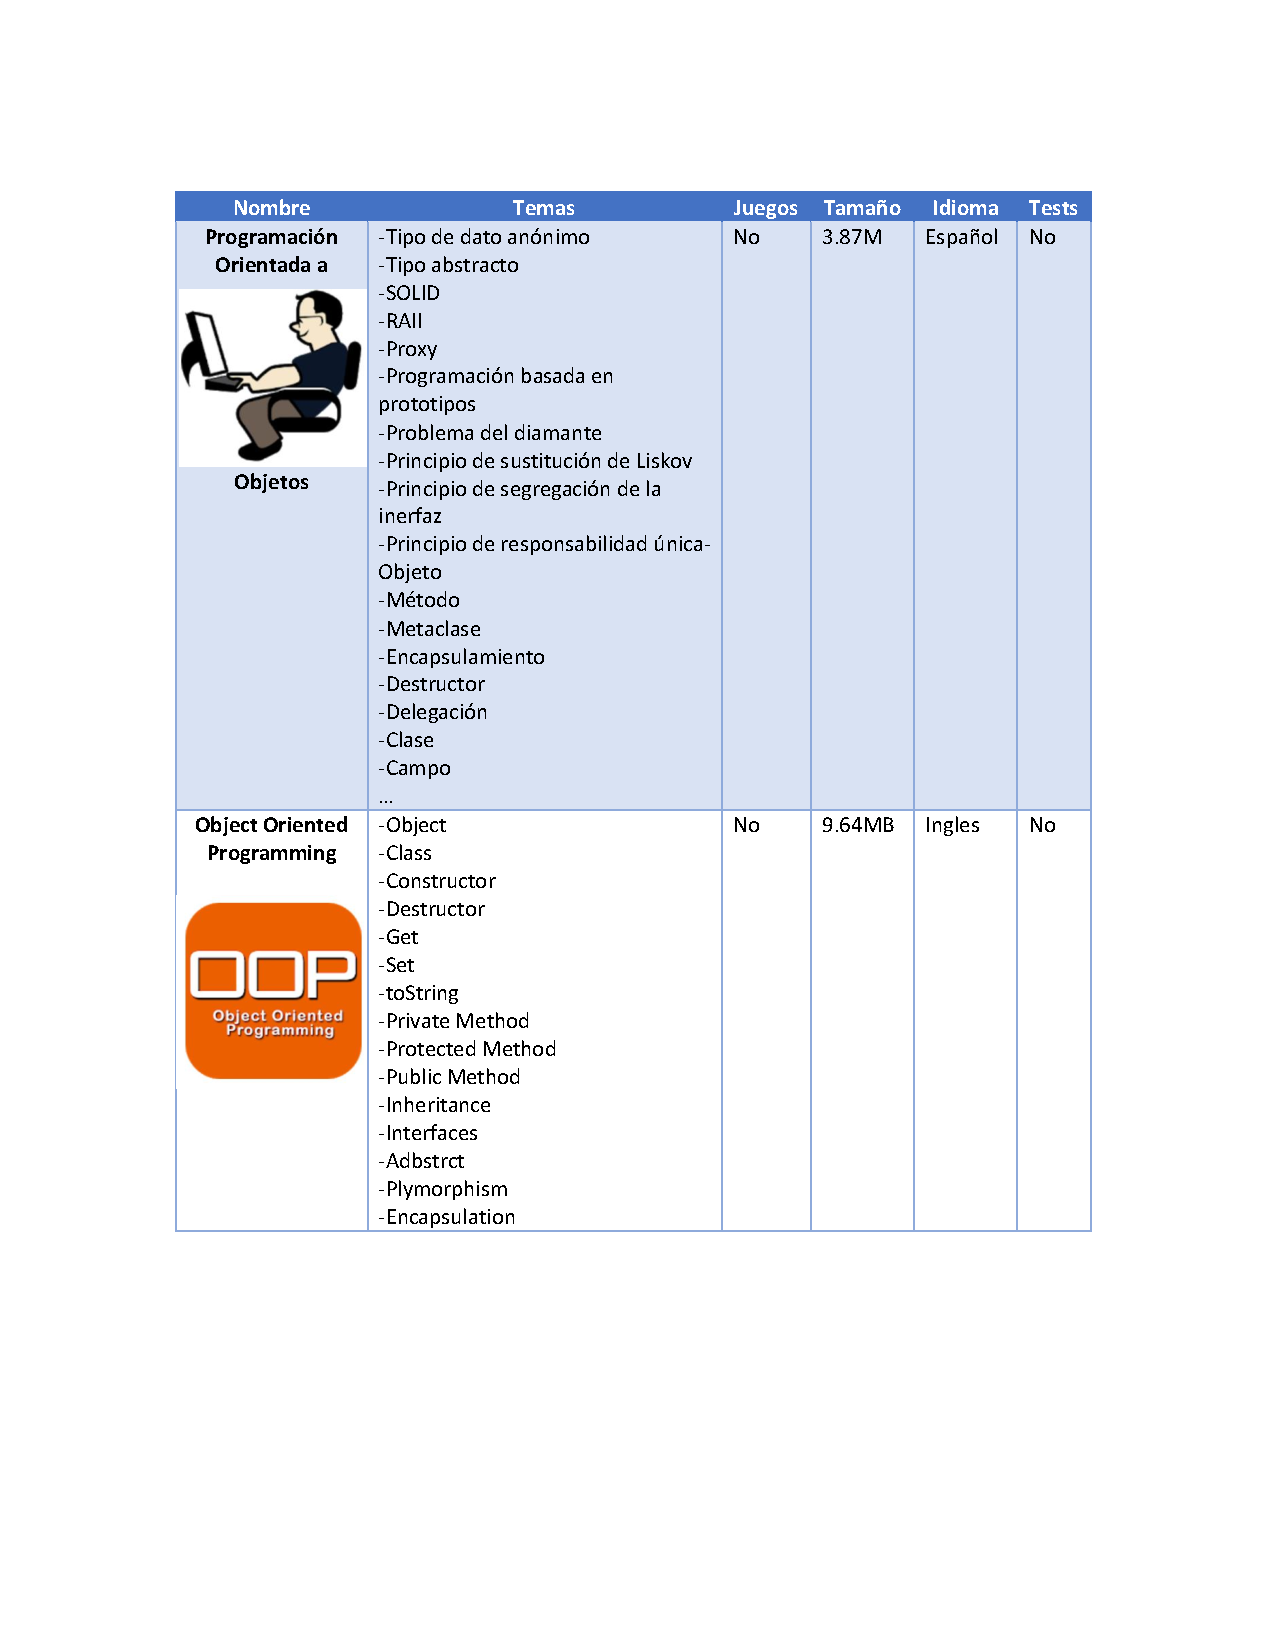
\includepdf{arte.pdf}

